\textbf{Partie A}

\begin{enumerate}
\item Le complément de l'arbre : on a au premier niveau :

$P(E) = \dfrac{25}{100} = 0,25,\quad P(F) = \dfrac{15}{100} = 0,15$, donc par complément à 1 : 

$P(C) = 1 - (0,25 + 0,15) = 1 - 0,4 = 0,6 = \dfrac{60}{100} = 60\,\%$.

Au second niveau :
\begin{itemize}
\item On sait que $ P_E(H) = 0,45$, d'où $P_E\left(\overline{H} \right)  = 1 - 0,45 = 0,55$ ;
\item $P_C(H) = 0,30$ d'où $P_C(H)  = 1 - 0,30 = 0,70$;

\end{itemize}

L'arbre de probabilités complété est :

\hfill
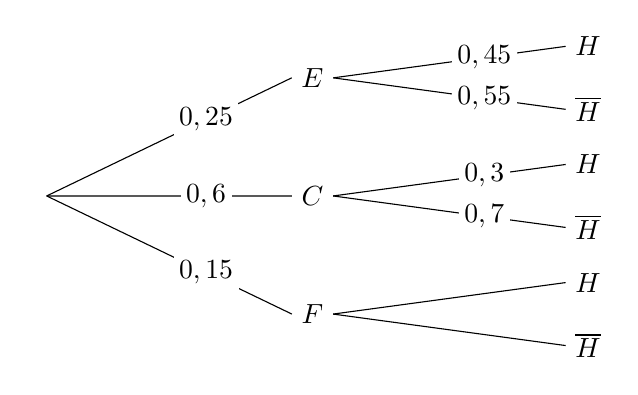
\begin{tikzpicture}[baseline={(R.center)},
	grow=right,
	level 1/.style={sibling distance=1.5cm,level distance=3.5cm},
	level 2/.style={sibling distance=0.8cm, level distance=3.5cm},
	edge from parent path={(\tikzparentnode.east) -- (\tikzchildnode.west)},
	every node/.style={},]
	\node (R){}
	child { node {$F$}
		child { node {$\overline{H}$} edge from parent}
		child { node {$H$} edge from parent}
		edge from parent node[pos=0.65,fill=white,inner sep=2pt]{$0,15$}}
	child { node {$C$}
		child { node {$\overline{H}$} edge from parent node[pos=0.65,fill=white,inner sep=2pt]{$0,7$}}
		child { node {$H$} edge from parent node[pos=0.65,fill=white,inner sep=2pt]{$0,3$}}
		edge from parent node[pos=0.65,fill=white,inner sep=2pt]{$0,6$}}
	child { node {$E$}
		child { node {$\overline{H}$} edge from parent node[pos=0.65,fill=white,inner sep=2pt]{$0,55$}}
		child { node {$H$} edge from parent node[pos=0.65,fill=white,inner sep=2pt]{$0,45$}}
		edge from parent node[pos=0.65,fill=white,inner sep=2pt]{$0,25$}};
\end{tikzpicture}\hfill~

\item Par définition des probabilités conditionnelles :

$P(E \cap H) = P(E) \times P_E(H)= 0,25 \times 0,45 = \np{0,1125}$.
\item Les évènements $E$, $C$ et $F$ forment une partition de l'univers, donc, d'après la formule des probabilités totales :

\quad $P(H) = P\big(\,E\cap H\big) + P\big(\,C\cap H\big) + P\big(\,F\cap H\big) $

D'où :\quad $\begin{aligned}[t] P(H)& = 0,1125 + P(C) \times P_C(H) +P\big(\,F\cap H\big) \\
			& = \np{0,1125} + 0,6 \times 0,3 + 0,12\\
			&= \np{0,1125} + 0,18 + 0,12\\
			& = \np{0,4125}
		\end{aligned} $

La probabilité qu'un abonné ait activé l'option \og Écoute hors-ligne\fg{} est bien de \np{0,4125}.
\item Trouver la probabilité qu'un abonné ayant activé l'option \og Écoute hors-ligne\fg{} ait choisi l'abonnement \og Étudiant\fg{} revient à calculer la probabilité $P_H(E)$.

$P_H(E)=\dfrac{P\big(\,H\cap E\big)}{P(H)}= \dfrac{\np{0,1125}}{\np{0,4152}} = \dfrac{3}{11} \approx 0,273 \quad\text{ à }10^{-3} \text{ près.}$

La probabilité qu'un abonné ayant activé l'option \og Écoute hors-ligne\fg{} ait choisi l'abonnement \og Étudiant\fg{} est égale à $0,273$ arrondi au millième.
\end{enumerate}

\textbf{Partie B}

\begin{enumerate}
\item On choisit huit abonnés de cette plateforme, au hasard et on considère qu'il y a suffisamment d'abonnés pour que ce choix soit assimilé à un tirage avec remise, c'est-à-dire à huit répétitions identiques et indépendantes.

La probabilité du succès (un abonné ait activé l'option \og Écoute hors-ligne\fg{}) est égale à \np{0,4125}.

Donc la variable aléatoire $X$ suit une loi binomiale de paramètres $n=8$ et $p= \np{0,4125}$.

\emph{Remarque :} ici, on a une rédaction plus légère, car l'énoncé demande d'admettre que $X$ suit une loi binomiale. Sinon, il faudrait les trois arguments classiques :

\begin{itemize}
\item On a une épreuve à deux issues, succès de probabilité $p = \np{0,4125}$ et échec;
\item cette épreuve est répétée $n = 8$ fois, de façon identique et indépendante (car la constitution de l'échantillon est assimilé à un tirage au sort \textbf{avec} remise);
\item $X$ est la variable aléatoire qui compte le nombre de succès sur ces $n$ répétitions.
\end{itemize}

\item Calculer la probabilité qu'aucun de ces huit abonnés n'ait activé l'option \og Écoute hors-ligne \fg{} revient à calculer la probabilité $P(X =0)$.

$\displaystyle P(X = 0)= \binom{8}{0} \times \np{0,4125}^0 \times (1 - \np{0,4125})^{8-0} = \np{0,5875}^8 \approx 0,014 \quad\text{ à } 10^{-3} \text{ près.}$

La probabilité qu'aucun de ces huit abonnés n'ait activé l'option \og Écoute hors-ligne \fg{} est de 0,014 arrondi au millième.

\item
	\begin{enumerate}
		\item Pour tout entier naturel non nul $n$, soit $X_n$ la variable aléatoire donnant le nombre d'abonnés ayant activé l'option \og Écoute hors-ligne \fg{}.

La variable aléatoire $X_n$ suit donc une loi binomiale de paramètres $n$ et $\np{0,4125}$.

$\displaystyle q_n = P(X_n \geqslant 1) = 1 - P (X_n=0) =1- \binom{n}{0} \times \np{0,4125}^0 \times (1- \np{0,4152})^{n-0}= 1- \np{0,5875}^n$.

Pour tout $n$ entier naturel non nul, on a bien \quad $q_{n}=1- \np{0,5875}^{n}$.

		\item Déterminer la plus petite valeur de $n$ telle que la probabilité qu'au moins un abonné de l'échantillon ait activé l'option \og Écoute hors-ligne\fg{} soit supérieure ou égale à $99,9\,\%$ revient à déterminer le plus petit entier naturel $n$ tel que $q_n \geqslant 0,999$.

$\begin{aligned}
q_n \geqslant 0,999 & \iff 1-\np{0,5875}^{n} \geqslant0,999 \\
& \iff 0,001 \geqslant \np{0,5875}^n \\
& \iff \ln(0,001) \geqslant \ln (\np{0,5875}^n) \quad \text{car la fonction logarithme népérien est croissante sur} ]0~;~+\infty[\\
& \iff \ln(0,001) \geqslant n\ln (\np{0,5875}) \quad \text{par propriété de la fonction ln}\\
& \iff \dfrac{\ln(0,001)}{\ln(\np{0,5875})} \leqslant n \quad \text{ car } \ln(\np{0,5875}) < 0
\end{aligned}$

Or $\dfrac{\ln(0,001)}{\ln(\np{0,5875})} \approx \np{12,9875}$

La plus petite valeur de $n$ telle que la probabilité qu'au moins un abonné de l'échantillon ait activé l'option \og Écoute hors-ligne\fg{} soit supérieure ou égale à $99,9\,\%$ est donc égale à~13.
	\end{enumerate}
\end{enumerate}

	\textbf{Partie C}

	\begin{enumerate}
	\item La variable aléatoire $Y$ peut prendre les valeurs :
	\begin{itemize}
		\item 5~\euro{} (uniquement l'abonnement \og Étudiant\fg{})
		\item 7~\euro{} (uniquement l'abonnement \og Étudiant\fg{} avec l'option \og Écoute hors-ligne\fg{} )
		\item 10~\euro{} (uniquement l'abonnement \og Classique \fg{})
		\item 12~\euro{} (uniquement l'abonnement \og Classique \fg{} avec l'option \og Écoute hors-ligne\fg{} )
		\item 16~\euro{} (uniquement l'abonnement \og Famille \fg{})
		\item 18~\euro{} (uniquement l'abonnement \og Famille \fg{} avec l'option \og Écoute hors-ligne\fg{} )
	\end{itemize}
	\item Il reste à calculer $P(F \cap H)$.
	
On a $P(F) = P(F \cap H) + P\left(F \cap \overline{H}\right) \iff 0,15 =  0,12 + P\left(F \cap \overline{H}\right) \iff P\left(F \cap \overline{H}\right) = 0,15 - 0,12 = 0,03$. Le tableau décrivant la loi de probabilité de la variable aléatoire $Y$ est donc :

\hfill~
\begin{tblr}{hlines, vlines, column{2-7}={1.2cm,c}}
	$y_i$& 5 & 7 & 10 & 12 & 16 & 18\\
	évènement $\left\{Y = y_i\right\}$& $E \cap \overline{H}$&$E \cap H$&$C \cap \overline{H}$&$C \cap H$&$F \cap \overline{H}$&$F \cap H$\\
	$P(Y = y_i)$&$0,1375$ & $0,1125$ & $0,42$ & $0,18$ & $0,03$ & $0,12$
\end{tblr}
\hfill~

\item $\begin{aligned}[t]
E(Y) &= \displaystyle \sum_{i=1}^{6}P(Y=y_i)y_i \\
	 &= 5 \times 0,1375 + 7 \times 0,1125 + 10 \times 0,42 + 12 \times 0,18 + 16 \times 0,03 + 18 \times 0,12\\	 &=10,475
\end{aligned}$

Ce qui est le résultat donné.

Sur un très grand nombre d'abonnés, le tarif moyen mensuel sera de 10,475~\euro{}.

\item À l'aide de la calculatrice, on trouve : $V(Y) \approx 13,70$ arrondi au centième.


\item
	\begin{enumerate}
		\item $V(Z) = \big(\sigma(Z)\big)^2= 2^2 =4$

La variance de la variable aléatoire $Z$ vaut 4.
		\item On cherche la probabilité que le prix de son abonnement soit strictement compris entre 6 et 12 euros soit $P(6 < Z <12)$

On remarque que l'espérance de $Z$ est $9$~\euro{}, c'est la valeur au milieu de l'intervalle $]6~;~12[$.

On a donc :\quad $\begin{aligned}[t]
	P(6 < Z <12)
	&= P(9-3<Z<9+3) \\
	&= P(-3 < Z-9 < 3)\\
	&= P\Big(\big|Z-9\big| < 3\Big)\\
	&= 1 - P(|Z-9|\geqslant 3)
\end{aligned}$

Or, pour tout réel $t > 0$, d'après l'inégalité de Bienaymé-Tchebychev, on a :

$P\Big(\big|Z-E(Z)\big| \geqslant t\Big) \leqslant \dfrac{V(Z)}{t^2}$

Pour $t = 3$ on obtient : \quad $ P\Big(\big|Z-9\big| \geqslant 3\Big)\leqslant \dfrac{4}{ 3^2}$.

D'où :\quad $1- P\Big(\big|Z-9\big| \geqslant 3\Big)\geqslant 1- \dfrac{4}{9}$.

Soit :\quad $P(6 <Z <12) \geqslant \dfrac{5}{9} > \dfrac{4,5}{9} = 0,5$.

Donc le responsable a raison, si on interroge un abonné de cette plateforme vidéo au hasard, il y a au moins $50\,\%$ de chances pour que le prix de son abonnement soit strictement compris entre 6 et 12 euros.
	\end{enumerate}
\end{enumerate}
